In this section we are going to present the strategy that the development team should use to implement \projectname~system. As we can see in the Component Dependency Diagram all the system's components have been created in such a way that they can be perfectly developed in parallels with the right dependency. All the components that are in the same column of the graph can be easily implemented together. Following this process, every time that a component need an interface from another one, it should been already implemented. However, this development strategy would lead to build a testable system only at the end, following a waterfall model, because the Meeting Controller component, that is the main component that manages meeting, would be implemented almost at the end of the process. This model doesn't fit with the modern correct implementation strategies because it will not show any prototype (alpha and beta versions) until the end of the process, denying the possibility of corrections and modifications on the go.\\

\begin{figure}[!h]
	\centering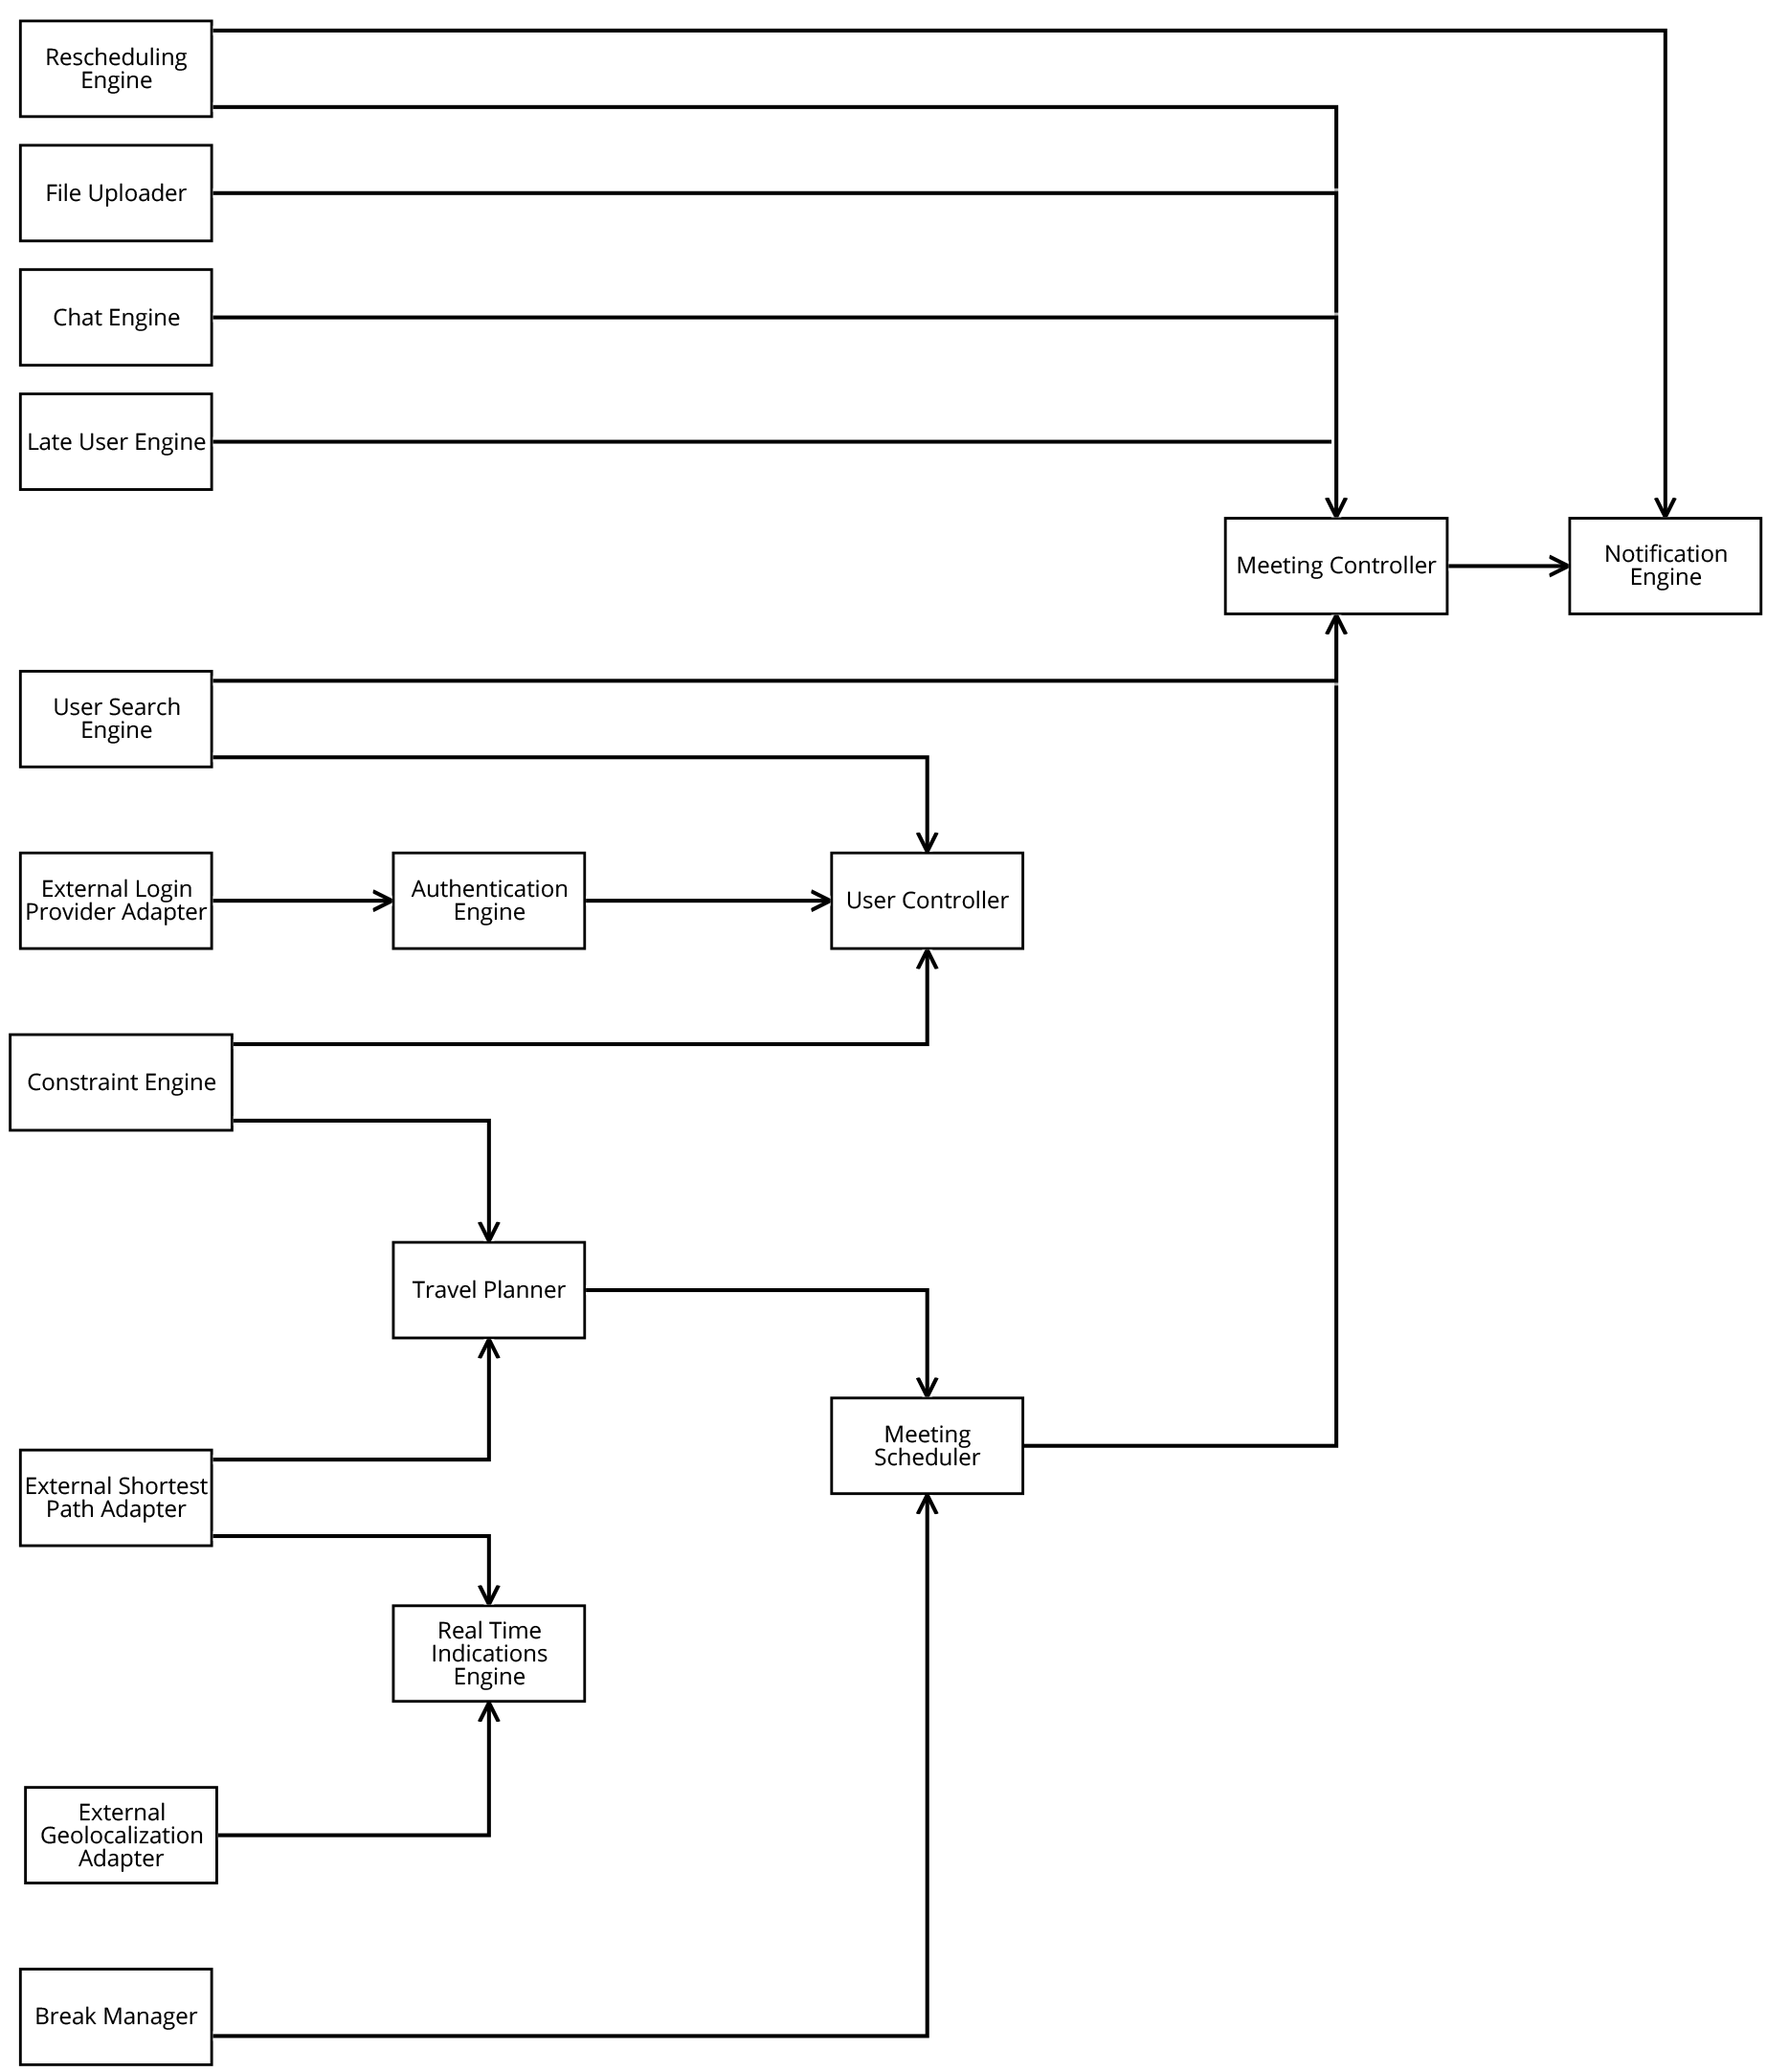
\includegraphics[scale = 0.22]{Images/UMLDiagrams/DependencyDiagram.png}
	\caption{Component Dependency Diagram}
\end{figure}

For this reason the best way to complete \projectname~ project is:
\begin{itemize}
	\item Develop Constraint Engine, External Shortest Path Adapter and Break Manager in order to have a complete background for the future development of other components.
	\item Develop Travel Planner component and integrate it with Constraint Engine and External Shortest Path Adapter following the integration test of the next chapters.
	\item Develop Meeting Scheduler component 
\end{itemize}

\clearpage